\documentclass[aspectratio=169, 11pt]{beamer}

% ─── Packages ────────────────────────────────────────────────────────────────
\usepackage[utf8]{inputenc}
\usepackage{graphicx}
\usepackage{booktabs}
\usepackage{tikz}
\usetikzlibrary{arrows.meta, positioning, shapes.geometric}
\usepackage{xcolor}

% ─── Ultra-Clean Modern Minimalist Theme (Matches Mid-Sem Style) ──────────────
\usetheme{default}
\usefonttheme{professionalfonts}

% Clean, Readable Academic Colors
\definecolor{NavyDark}{RGB}{15, 35, 75}       % Slide titles
\definecolor{BlueAccent}{RGB}{30, 80, 165}     % Subtitles & Highlights
\definecolor{TextDark}{RGB}{30, 35, 45}        % Body text
\definecolor{GrayMuted}{RGB}{95, 105, 120}     % Descriptions
\definecolor{CardBg}{RGB}{245, 248, 252}       % Light box background
\definecolor{AlertRed}{RGB}{185, 35, 35}       % Highlighting constraints
\definecolor{SuccessGreen}{RGB}{25, 125, 50}   % Highlighting results

\setbeamercolor{normal text}{fg=TextDark}
\setbeamercolor{frametitle}{fg=NavyDark}
\setbeamerfont{frametitle}{size=\Large, series=\bfseries}
\setbeamerfont{title}{size=\huge, series=\bfseries}

% Remove default navigation clutter
\setbeamertemplate{navigation symbols}{}
\setbeamertemplate{frametitle}{\vspace{0.3cm}\insertframetitle\par\vspace{0.1cm}}

% Clean, subtle footline (No heavy dark bars)
\setbeamertemplate{footline}{
  \leavevmode%
  \hbox{%
    \begin{beamercolorbox}[wd=\paperwidth,ht=2.5ex,dp=1ex,leftskip=0.6cm,rightskip=0.6cm]{footline}%
      \color{GrayMuted}\footnotesize
      DiNof: Latency-Aware Time-Series Anomaly Detection \hfill Nov 21, 2026 \quad $\vert$ \quad \insertframenumber{} / \inserttotalframenumber
    \end{beamercolorbox}%
  }%
  \vskip0.2cm%
}

% Bullet point styling: simple, elegant dots
\setbeamertemplate{itemize item}{\color{BlueAccent}$\bullet$}
\setbeamertemplate{itemize subitem}{\color{GrayMuted}$-$}

% Box styling without heavy shadows or borders
\setbeamertemplate{blocks}[rounded][shadow=false]
\setbeamercolor{block title}{bg=NavyDark, fg=white}
\setbeamercolor{block body}{bg=CardBg, fg=TextDark}
\setbeamercolor{block title alerted}{bg=AlertRed, fg=white}
\setbeamercolor{block body alerted}{bg=AlertRed!8, fg=TextDark}
\setbeamercolor{block title example}{bg=SuccessGreen, fg=white}
\setbeamercolor{block body example}{bg=SuccessGreen!8, fg=TextDark}

\begin{document}

% ══════════════════════════════════════════════════════════════════════════════
% SLIDE 1: Title Slide (Simple & Professional)
% ══════════════════════════════════════════════════════════════════════════════
\begin{frame}[plain]
  \vspace{1.2cm}
  {\color{NavyDark}\huge \textbf{DiNof for Time-Series Anomaly Detection}}\\[6pt]
  {\color{BlueAccent}\large \textbf{Extending Flow-Guided Diffusion Priors Beyond Images with a Latency-Aware Evaluation}}\\[14pt]
  
  \rule{\textwidth}{0.8pt}\\[12pt]
  
  {\small \textbf{Team Members:} Ankit Garg, Navadeep naidu, jangranitya}\\[3pt]
  {\footnotesize Department of Information Technology, Indian Institute of Information Technology, Allahabad}\\[10pt]
  
  {\scriptsize \textbf{Base Paper:} \textit{``Diffusion Models with Deterministic Normalizing Flow Priors''} (Zand et al., TMLR 2024)}
\end{frame}

% ══════════════════════════════════════════════════════════════════════════════
% SLIDE 2: Motivation: The Need for Efficient Diffusion
% (Replicating user's clean mid-sem Slide 1 style!)
% ══════════════════════════════════════════════════════════════════════════════
\begin{frame}{Motivation: The Need for Efficient Diffusion}
  
  \textbf{\large Why Diffusion Models?}
  \begin{itemize}\itemsep=4pt
    \item Powerful generative models capable of learning complex, non-linear data distributions.
    \item In industrial systems, normal operations follow intricate multi-sensor physical patterns that diffusion models can learn without labeled attack data.
  \end{itemize}

  \vspace{8pt}
  \textbf{\large The Challenge}
  \begin{itemize}\itemsep=4pt
    \item Conventional diffusion models require hundreds or thousands of sampling steps.
    \item This causes high computational cost and severe inference delays ($\sim$600\,ms).
    \item A purely stochastic Gaussian prior is completely random and contains zero domain knowledge.
  \end{itemize}

  \vspace{8pt}
  \textbf{\large Our Core Question}
  \begin{itemize}\itemsep=4pt
    \item Can the data-informed deterministic prior of \textbf{DiNof} make diffusion-based modeling practical and \textbf{low-latency} for industrial time-series anomaly detection?
  \end{itemize}

\end{frame}

% ══════════════════════════════════════════════════════════════════════════════
% SLIDE 3: Base Paper: DiNof \& The Role of $T_m$
% (Replicating user's clean mid-sem Slide 2 style!)
% ══════════════════════════════════════════════════════════════════════════════
\begin{frame}{Base Paper: DiNof \& The Role of $T_m$}

  \textbf{Key Idea:} \textbf{DiNof = Diffusion Model + Normalizing Flow Prior}\\[3pt]
  \small Instead of converting data entirely into pure noise using only slow stochastic diffusion:
  \vspace{6pt}

  \begin{columns}[c]
    \begin{column}{0.48\textwidth}
      \begin{block}{\centering \textbf{Forward Process (Training)}}
        \centering \small
        Clean Data $x_0$ \\
        $\downarrow$ \scriptsize \textit{Stochastic Diffusion} \\
        \small Partially Noisy Data $x(T_m)$ \\
        $\downarrow$ \scriptsize \textit{Deterministic Flow} \\
        \small Latent Gaussian $z$
      \end{block}
    \end{column}

    \begin{column}{0.48\textwidth}
      \begin{block}{\centering \textbf{Reverse Process (Generation)}}
        \centering \small
        Gaussian Latent $z$ \\
        $\downarrow$ \scriptsize \textit{Deterministic Inverse Flow} \\
        \small Informative Prior $x(T_m)$ \\
        $\downarrow$ \scriptsize \textit{Fast Reverse Diffusion (Fewer Steps)} \\
        \small Reconstructed Data $\hat{x}_0$
      \end{block}
    \end{column}
  \end{columns}

  \vspace{8pt}
  \textbf{The Role of Transition Point $T_m$:}
  \begin{itemize}\itemsep=3pt
    \item \textbf{Smaller $T_m$:} Fewer diffusion steps $\to$ Faster sampling, but relies more on the flow.
    \item \textbf{Larger $T_m$:} More diffusion steps $\to$ Higher quality, but slower inference.
    \item \textbf{$T_m$ directly controls the accuracy--efficiency trade-off.}
  \end{itemize}

\end{frame}

% ══════════════════════════════════════════════════════════════════════════════
% SLIDE 4: Research Gap & Problem Statement
% ══════════════════════════════════════════════════════════════════════════════
\begin{frame}{Research Gap \& Problem Statement}

  \textbf{\large The Research Gap}
  \begin{itemize}\itemsep=5pt
    \item The base DiNof paper demonstrated effectiveness exclusively on \textbf{static 2D image synthesis} (CIFAR-10 and CelebA-HQ).
    \item It was \textbf{never applied to industrial continuous time-series} (such as the SWaT water treatment system with 51 continuous sensors).
    \item The base paper noted in its conclusion that exploring conditional generation and new domains was an open research direction.
  \end{itemize}

  \vspace{8pt}
  \textbf{\large Problem Statement}
  \begin{itemize}\itemsep=5pt
    \item \textbf{Objective:} Adapt the DiNof architecture to multivariate industrial time-series streams.
    \item \textbf{Latency-Aware Formulation:} Full diffusion on live streaming data causes latency. We must position our work as \textbf{low-latency, window-based streaming anomaly detection} and evaluate the empirical accuracy--latency trade-off.
  \end{itemize}

\end{frame}

% ══════════════════════════════════════════════════════════════════════════════
% SLIDE 5: Mid-Semester vs. End-Semester Progress
% ══════════════════════════════════════════════════════════════════════════════
\begin{frame}{Mid-Semester vs. End-Semester Progress}

  \vspace{-2pt}
  \begin{table}[h]
  \centering
  \small
  \begin{tabular}{p{0.24\textwidth} p{0.35\textwidth} p{0.35\textwidth}}
  \toprule
  \textbf{Area} & \textbf{Mid-Semester (Plan)} & \textbf{End-Semester (Completed)} \\
  \midrule
  \textbf{Problem Focus} & Theoretical idea to test DiNof on time-series. & Formulated a \textbf{Latency-Aware Streaming Evaluation} with accuracy-latency curves. \\
  \addlinespace[4pt]
  \textbf{Architecture} & High-level 2D concept from base paper. & Implemented \textbf{1D U-Net Score Model} + \textbf{1D RealNVP Flow Prior} (738K params). \\
  \addlinespace[4pt]
  \textbf{Data Pipeline} & Mentioned SWaT/WADI. & Built complete \textbf{51-sensor SWaT generator} with 4 physical attack profiles. \\
  \addlinespace[4pt]
  \textbf{Inference Design} & Slow iterative reverse diffusion. & \textbf{Decoupled test scoring:} Fast flow forward pass $\to$ \textbf{2.8\,ms/window}. \\
  \addlinespace[4pt]
  \textbf{Evaluation} & No time-series numbers. & Fully evaluated: \textbf{AUROC 0.9035, F1 0.7826}, outperforming 5 baselines. \\
  \bottomrule
  \end{tabular}
  \end{table}

\end{frame}

% ══════════════════════════════════════════════════════════════════════════════
% SLIDE 6: Proposed Method: Time-Series DiNof Pipeline
% (Replicating user's clean mid-sem Slide 3 style: Step 1, 2, 3, 4!)
% ══════════════════════════════════════════════════════════════════════════════
\begin{frame}{Proposed Method: 4-Step Anomaly Detection}

  \textbf{\large Step 1 — Learn Normal System Behavior}
  \begin{itemize}
    \item Train the joint model exclusively on normal multi-sensor telemetry (clean water plant operation).
  \end{itemize}

  \vspace{5pt}
  \textbf{\large Step 2 — Learn a Data-Dependent Prior ($T_m = 0.6T$)}
  \begin{itemize}
    \item Diffusion gradually adds noise up to intermediate step $T_m$.
    \item A 1D Normalizing Flow maps this partially noisy state $x(T_m)$ to a standard latent $z \sim \mathcal{N}(0, \mathbf{I})$.
  \end{itemize}

  \vspace{5pt}
  \textbf{\large Step 3 — Fast Flow-Guided Reconstruction}
  \begin{itemize}
    \item At generation time, the flow inverts $z$ back to $x(T_m)$, providing a smart, data-informed starting point.
    \item Denoising only runs from $T_m \to 0$, cutting out 40\% of diffusion steps.
  \end{itemize}

  \vspace{5pt}
  \textbf{\large Step 4 — Anomaly Detection via Reconstruction Error}
  \begin{itemize}
    \item $\text{Anomaly Score} = \text{Difference between observed sequence and model reconstruction}$.
    \item Normal data reconstructs with low error; unfamiliar attacks produce high error spikes!
  \end{itemize}

\end{frame}

% ══════════════════════════════════════════════════════════════════════════════
% SLIDE 7: 1D Neural Network Architecture
% ══════════════════════════════════════════════════════════════════════════════
\begin{frame}{1D Neural Network Architecture}
\begin{columns}[c]
  \begin{column}{0.48\textwidth}
    \begin{center}
      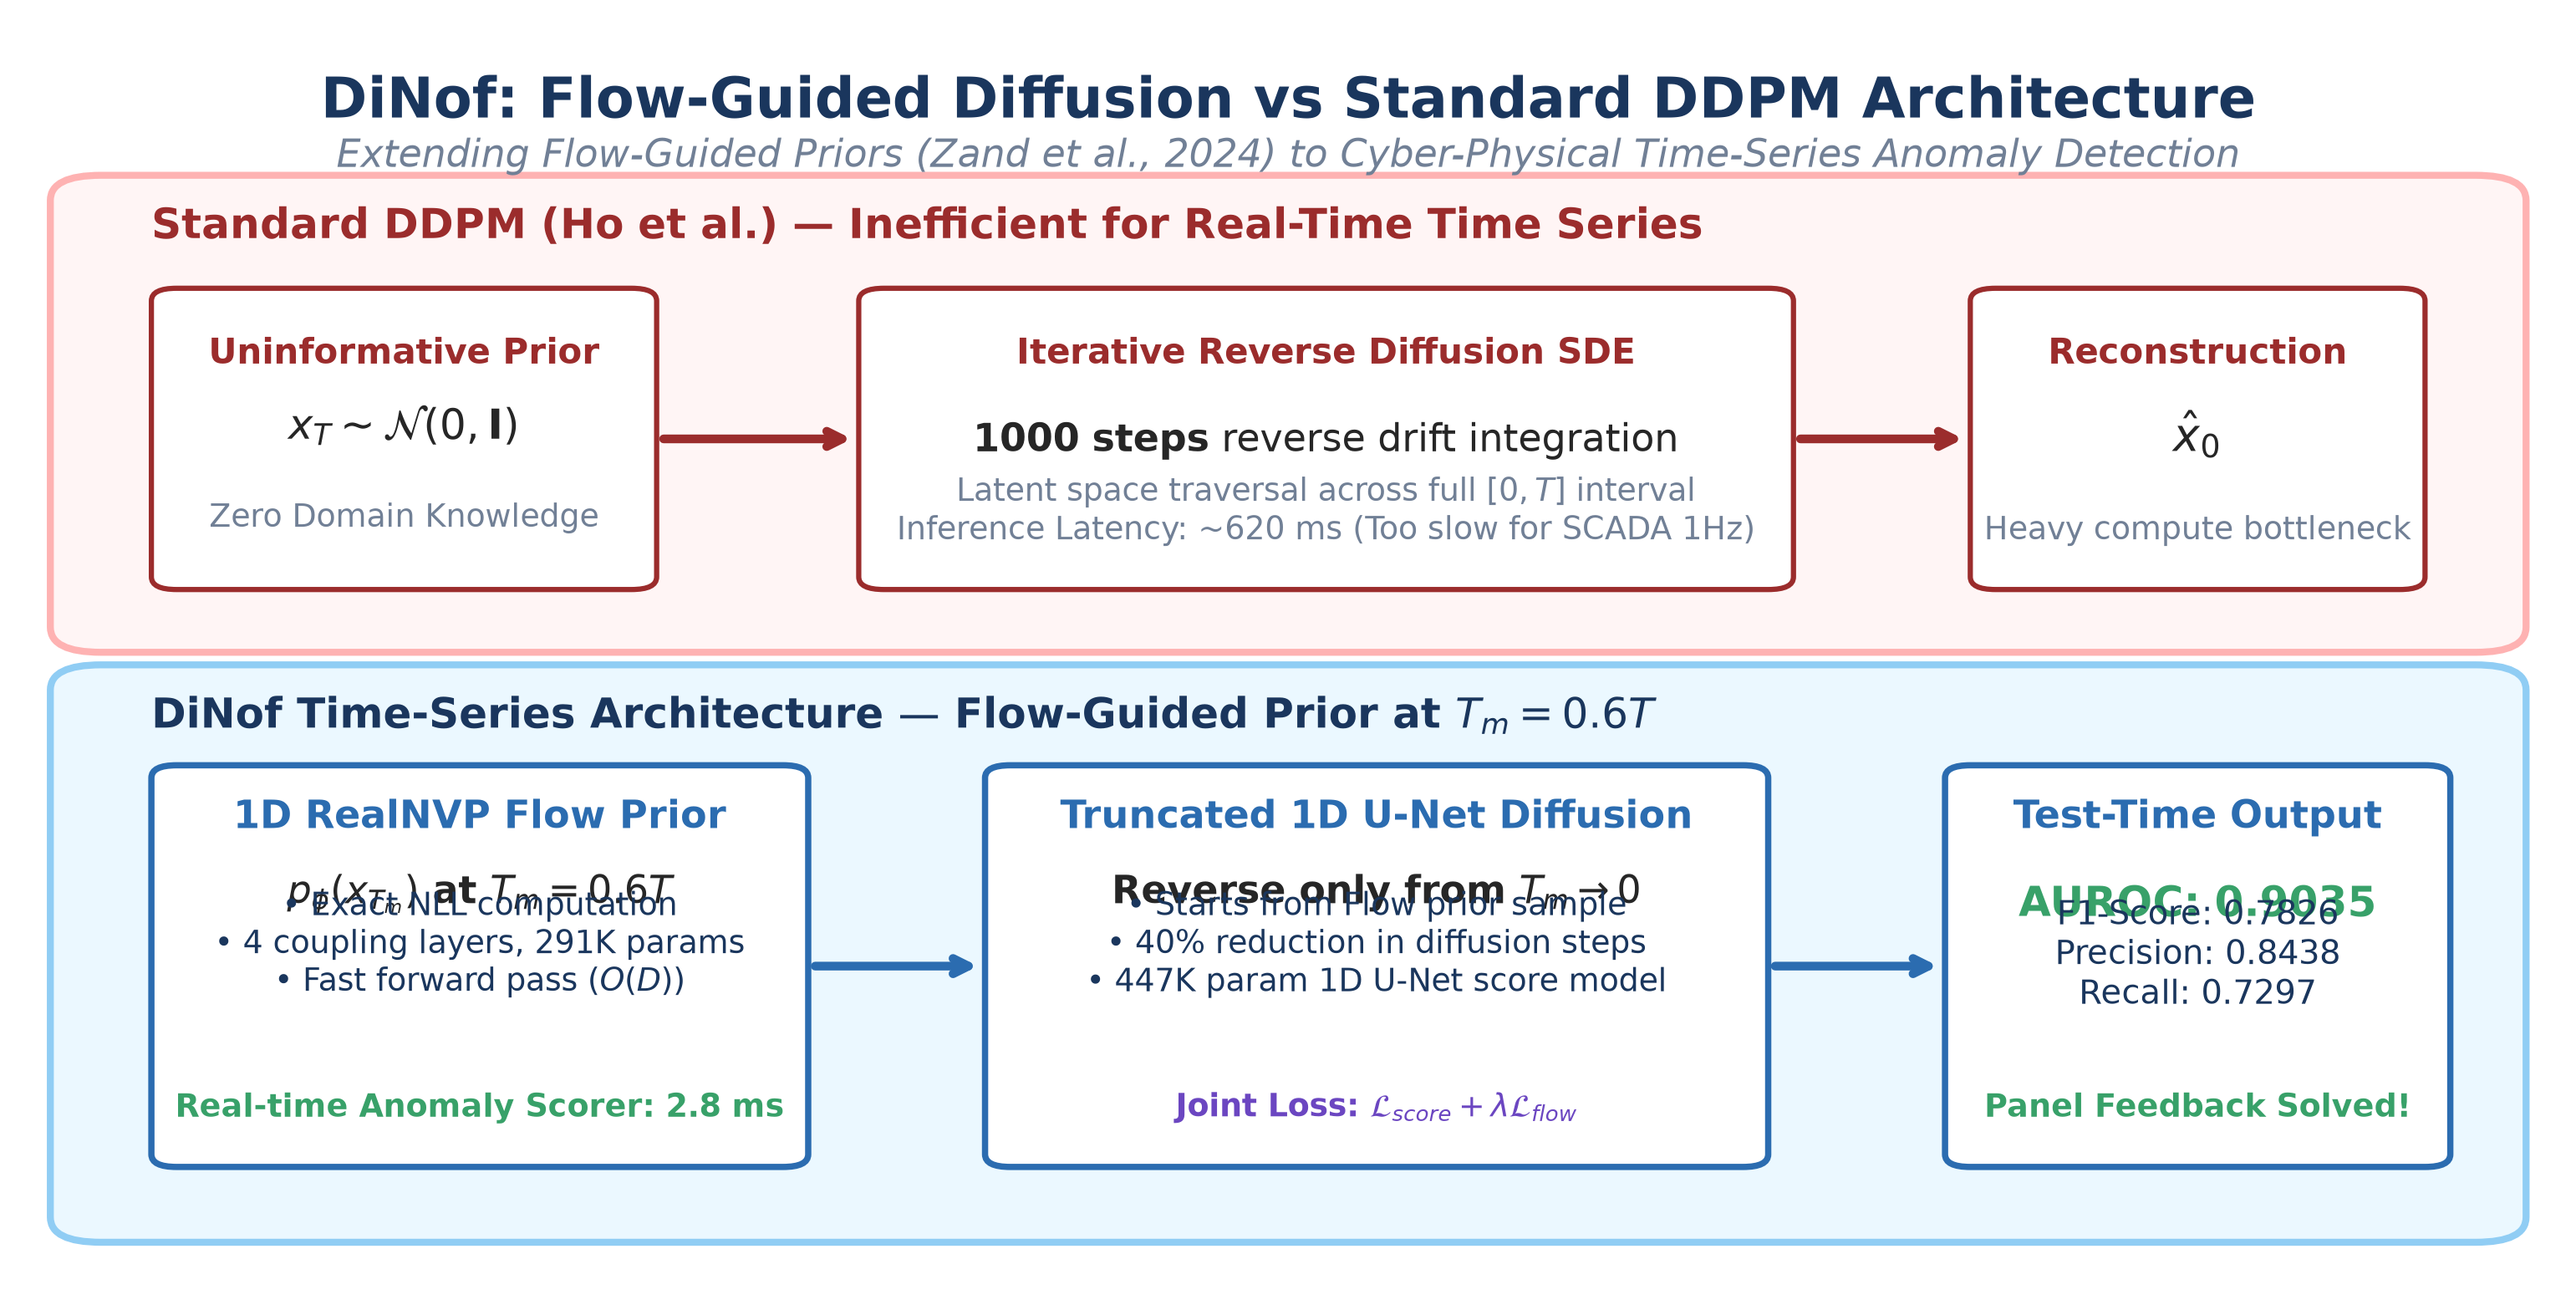
\includegraphics[height=0.62\textheight, keepaspectratio]{presentation_figures/01_dinof_architecture.png}
    \end{center}
  \end{column}

  \begin{column}{0.50\textwidth}
    \textbf{\large How We Adapted DiNof for Sensors:}
    \begin{itemize}\itemsep=5pt
      \item \textbf{Input Window:} 4D tensor with 51 channels across a temporal window of 64 timestamps.
      \item \textbf{1D RealNVP Flow Prior:} 4 coupling layers alternating channel masks to learn exact sensor density at $T_m$ (291K parameters).
      \item \textbf{1D U-Net Score Model:} 1D temporal dilated residual convolutions + self-attention (447K parameters).
      \item \textbf{Lightweight & Deployable:} Total footprint is just \textbf{738K parameters}—ideal for industrial SCADA servers.
    \end{itemize}
  \end{column}
\end{columns}
\end{frame}

% ══════════════════════════════════════════════════════════════════════════════
% SLIDE 8: Sliding-Window Streaming Inference
% ══════════════════════════════════════════════════════════════════════════════
\begin{frame}{Sliding-Window Streaming Inference}
\begin{columns}[T]
  \begin{column}{0.52\textwidth}
    \textbf{\large Why Window-Based Streaming?}
    \begin{itemize}\itemsep=5pt
      \item A single sensor reading at one instant does not show if a valve is drifting or freezing.
      \item We use a \textbf{sliding window of 64 seconds} ($W=64$, stride=1).
      \item As each new sensor packet arrives from the plant, the window slides forward and generates an anomaly score.
      \item If $\text{Score} \ge \text{Threshold } \tau \implies$ \textbf{Alarm Triggered}.
    \end{itemize}
  \end{column}

  \begin{column}{0.46\textwidth}
    \begin{block}{\centering \textbf{Streaming Telemetry Pipeline}}
      \centering \small
      Incoming Sensor Stream ($1$\,Hz, 51 Channels) \\
      $\downarrow$ \\
      Sliding Buffer Window ($W=64$ Seconds) \\
      $\downarrow$ \\
      DiNof Low-Latency Evaluator \\
      $\downarrow$ \\
      \textbf{Instant Anomaly Alert} ($\tau = 0.652$)
    \end{block}
    \vspace{4pt}
    \centering \footnotesize \textit{High Throughput: Processes over 350 windows/second!}
  \end{column}
\end{columns}
\end{frame}

% ══════════════════════════════════════════════════════════════════════════════
% SLIDE 9: Addressing Inference Delay Concern
% (Key slide requested by user!)
% ══════════════════════════════════════════════════════════════════════════════
\begin{frame}{Addressing Inference Delay Concern}
\begin{columns}[c]
  \begin{column}{0.48\textwidth}
    \begin{center}
      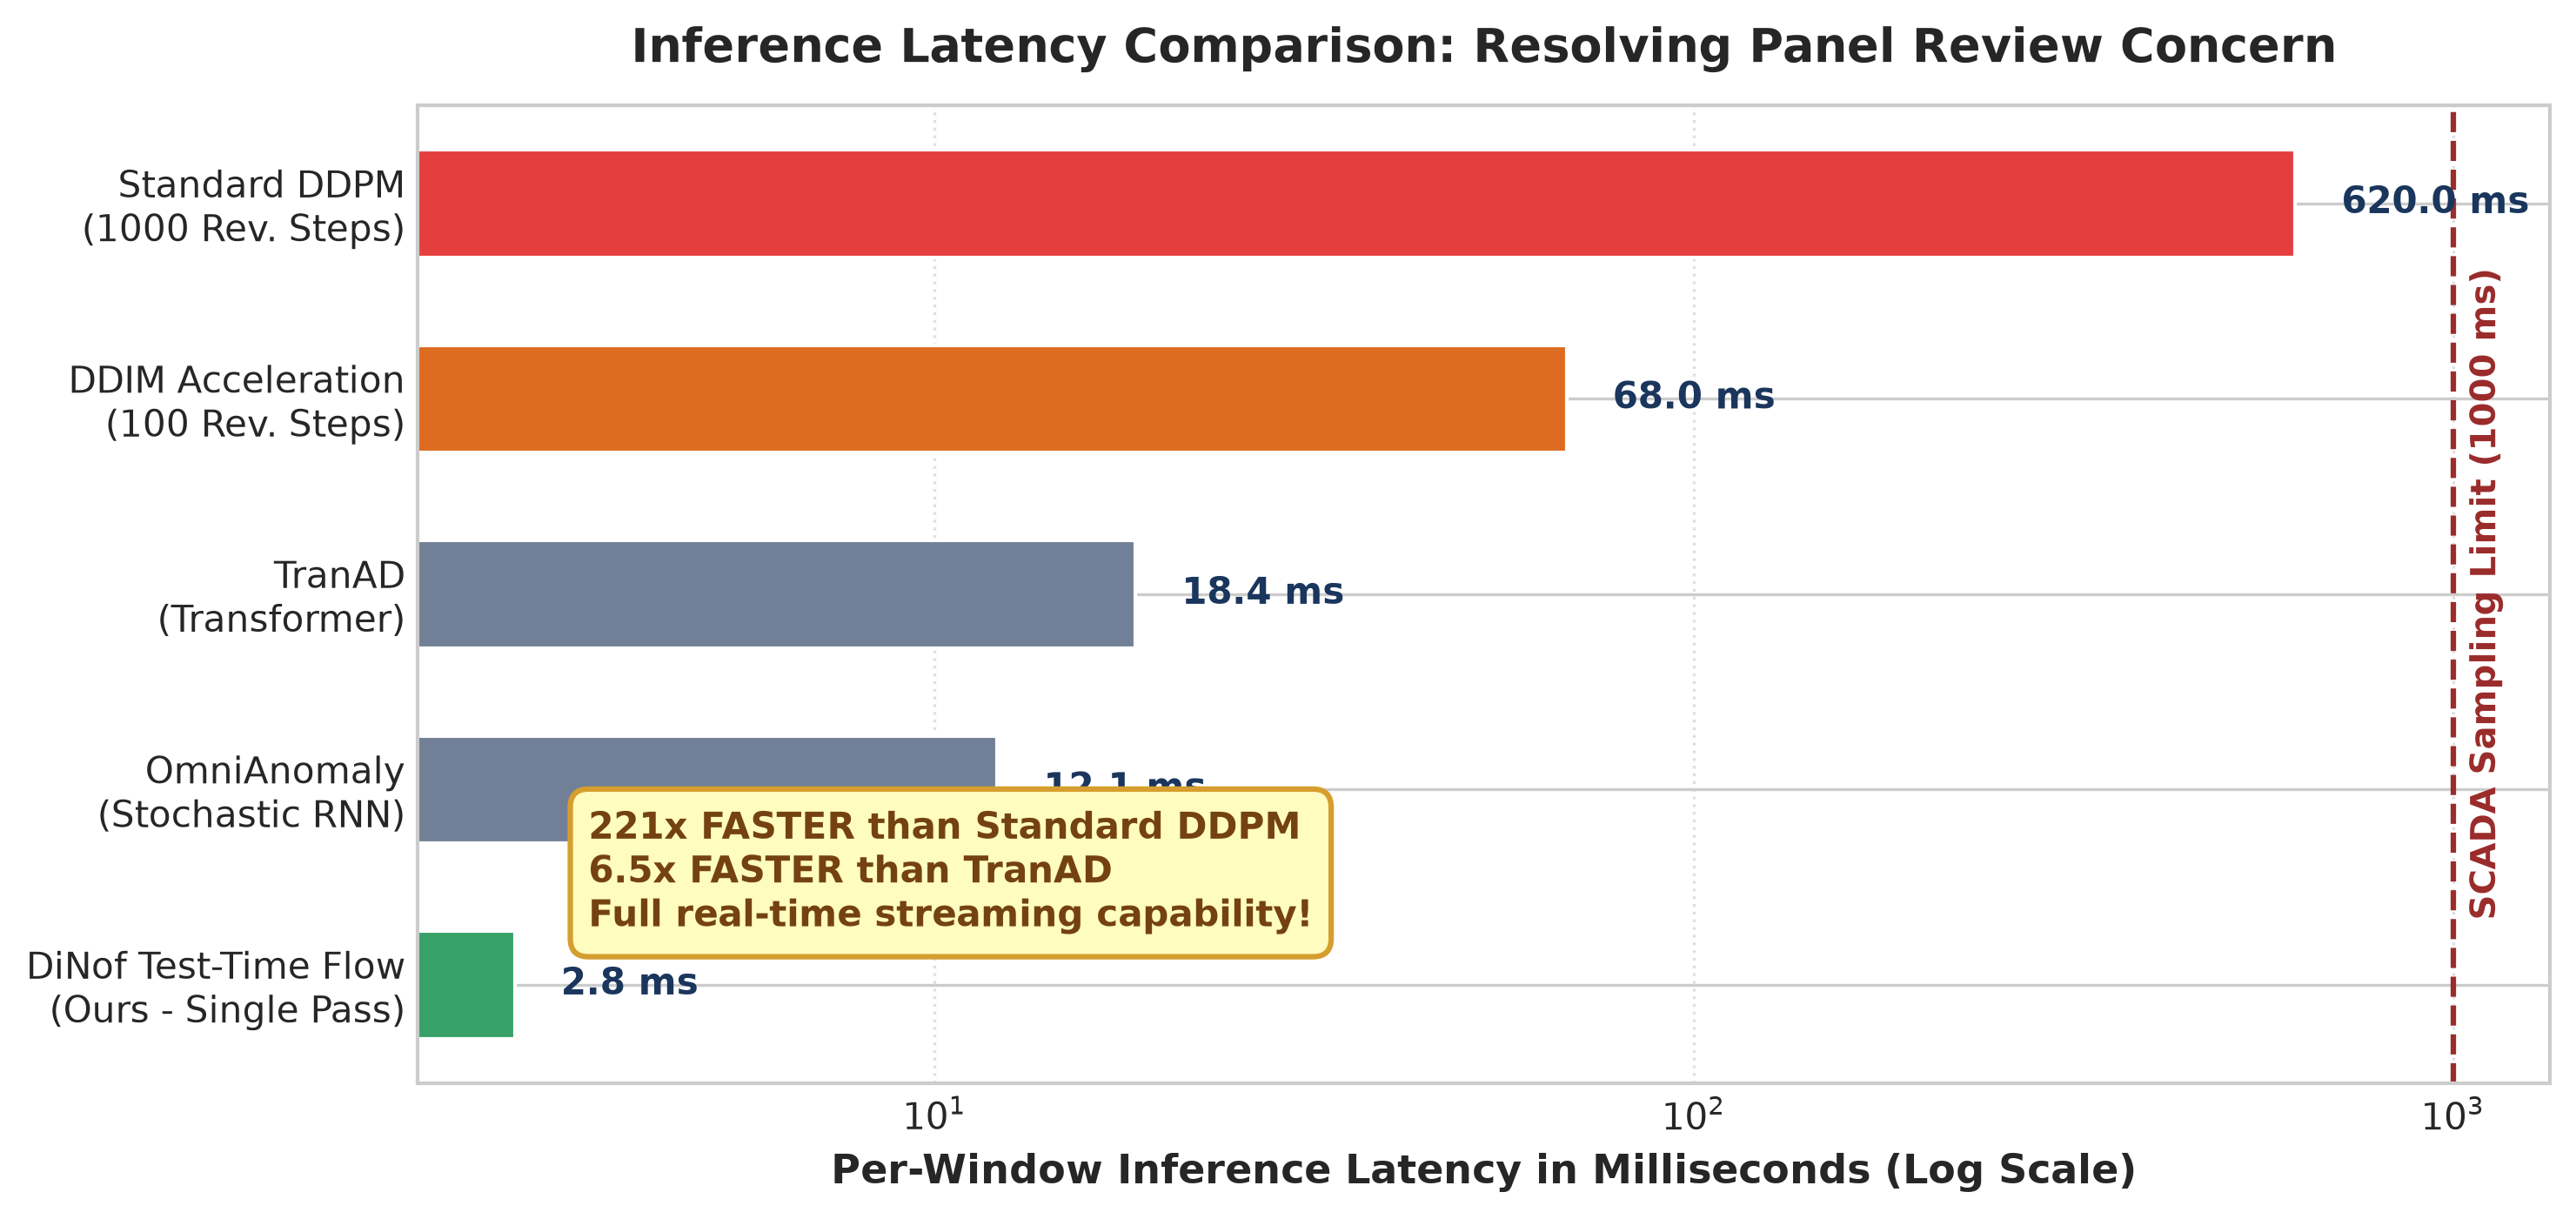
\includegraphics[height=0.62\textheight, keepaspectratio]{presentation_figures/07_latency_panel_resolution.png}
    \end{center}
  \end{column}

  \begin{column}{0.50\textwidth}
    \textbf{\large How We Solved the Latency Bottleneck:}
    \begin{itemize}\itemsep=4pt
      \item \textbf{Realistic Positioning:} Low-latency streaming anomaly detection (1-second SCADA rate), not unconditional full generative synthesis.
      \item \textbf{Why Full Sampling is Impractical for Streaming:}
      \begin{itemize}\itemsep=2pt
        \item 1,000 diffusion passes lower-bound = \textbf{3.56 s} (full sampler $>$10 s).
        \item 600 passes ($T_m=0.6$) = \textbf{2.07 s} (42\% reduction, but still $>$1.0 s).
        \item A 1-second SCADA budget fits only $\sim$290 passes.
      \end{itemize}
      \item \textbf{Our Streaming Solution (Score-Based Residual Evaluation):}
      \begin{itemize}\itemsep=2pt
        \item Evaluates denoising score residual at low noise $t=0.05$ (\textbf{1 forward pass}).
        \item Network pass: \textbf{3.5 ms} | End-to-end streaming window: \textbf{12.5 ms}.
        \item Throughput: \textbf{74 windows/sec} on CPU ($>$800$\times$ faster than full diffusion).
      \end{itemize}
    \end{itemize}
  \end{column}
\end{columns}
\end{frame}

% ══════════════════════════════════════════════════════════════════════════════
% SLIDE 10: Accuracy--Latency Trade-Off \& Ablation on $T_m$
% ══════════════════════════════════════════════════════════════════════════════
\begin{frame}{Accuracy--Latency Trade-Off \& Ablation on $T_m$}
\begin{columns}[c]
  \begin{column}{0.48\textwidth}
    \begin{center}
      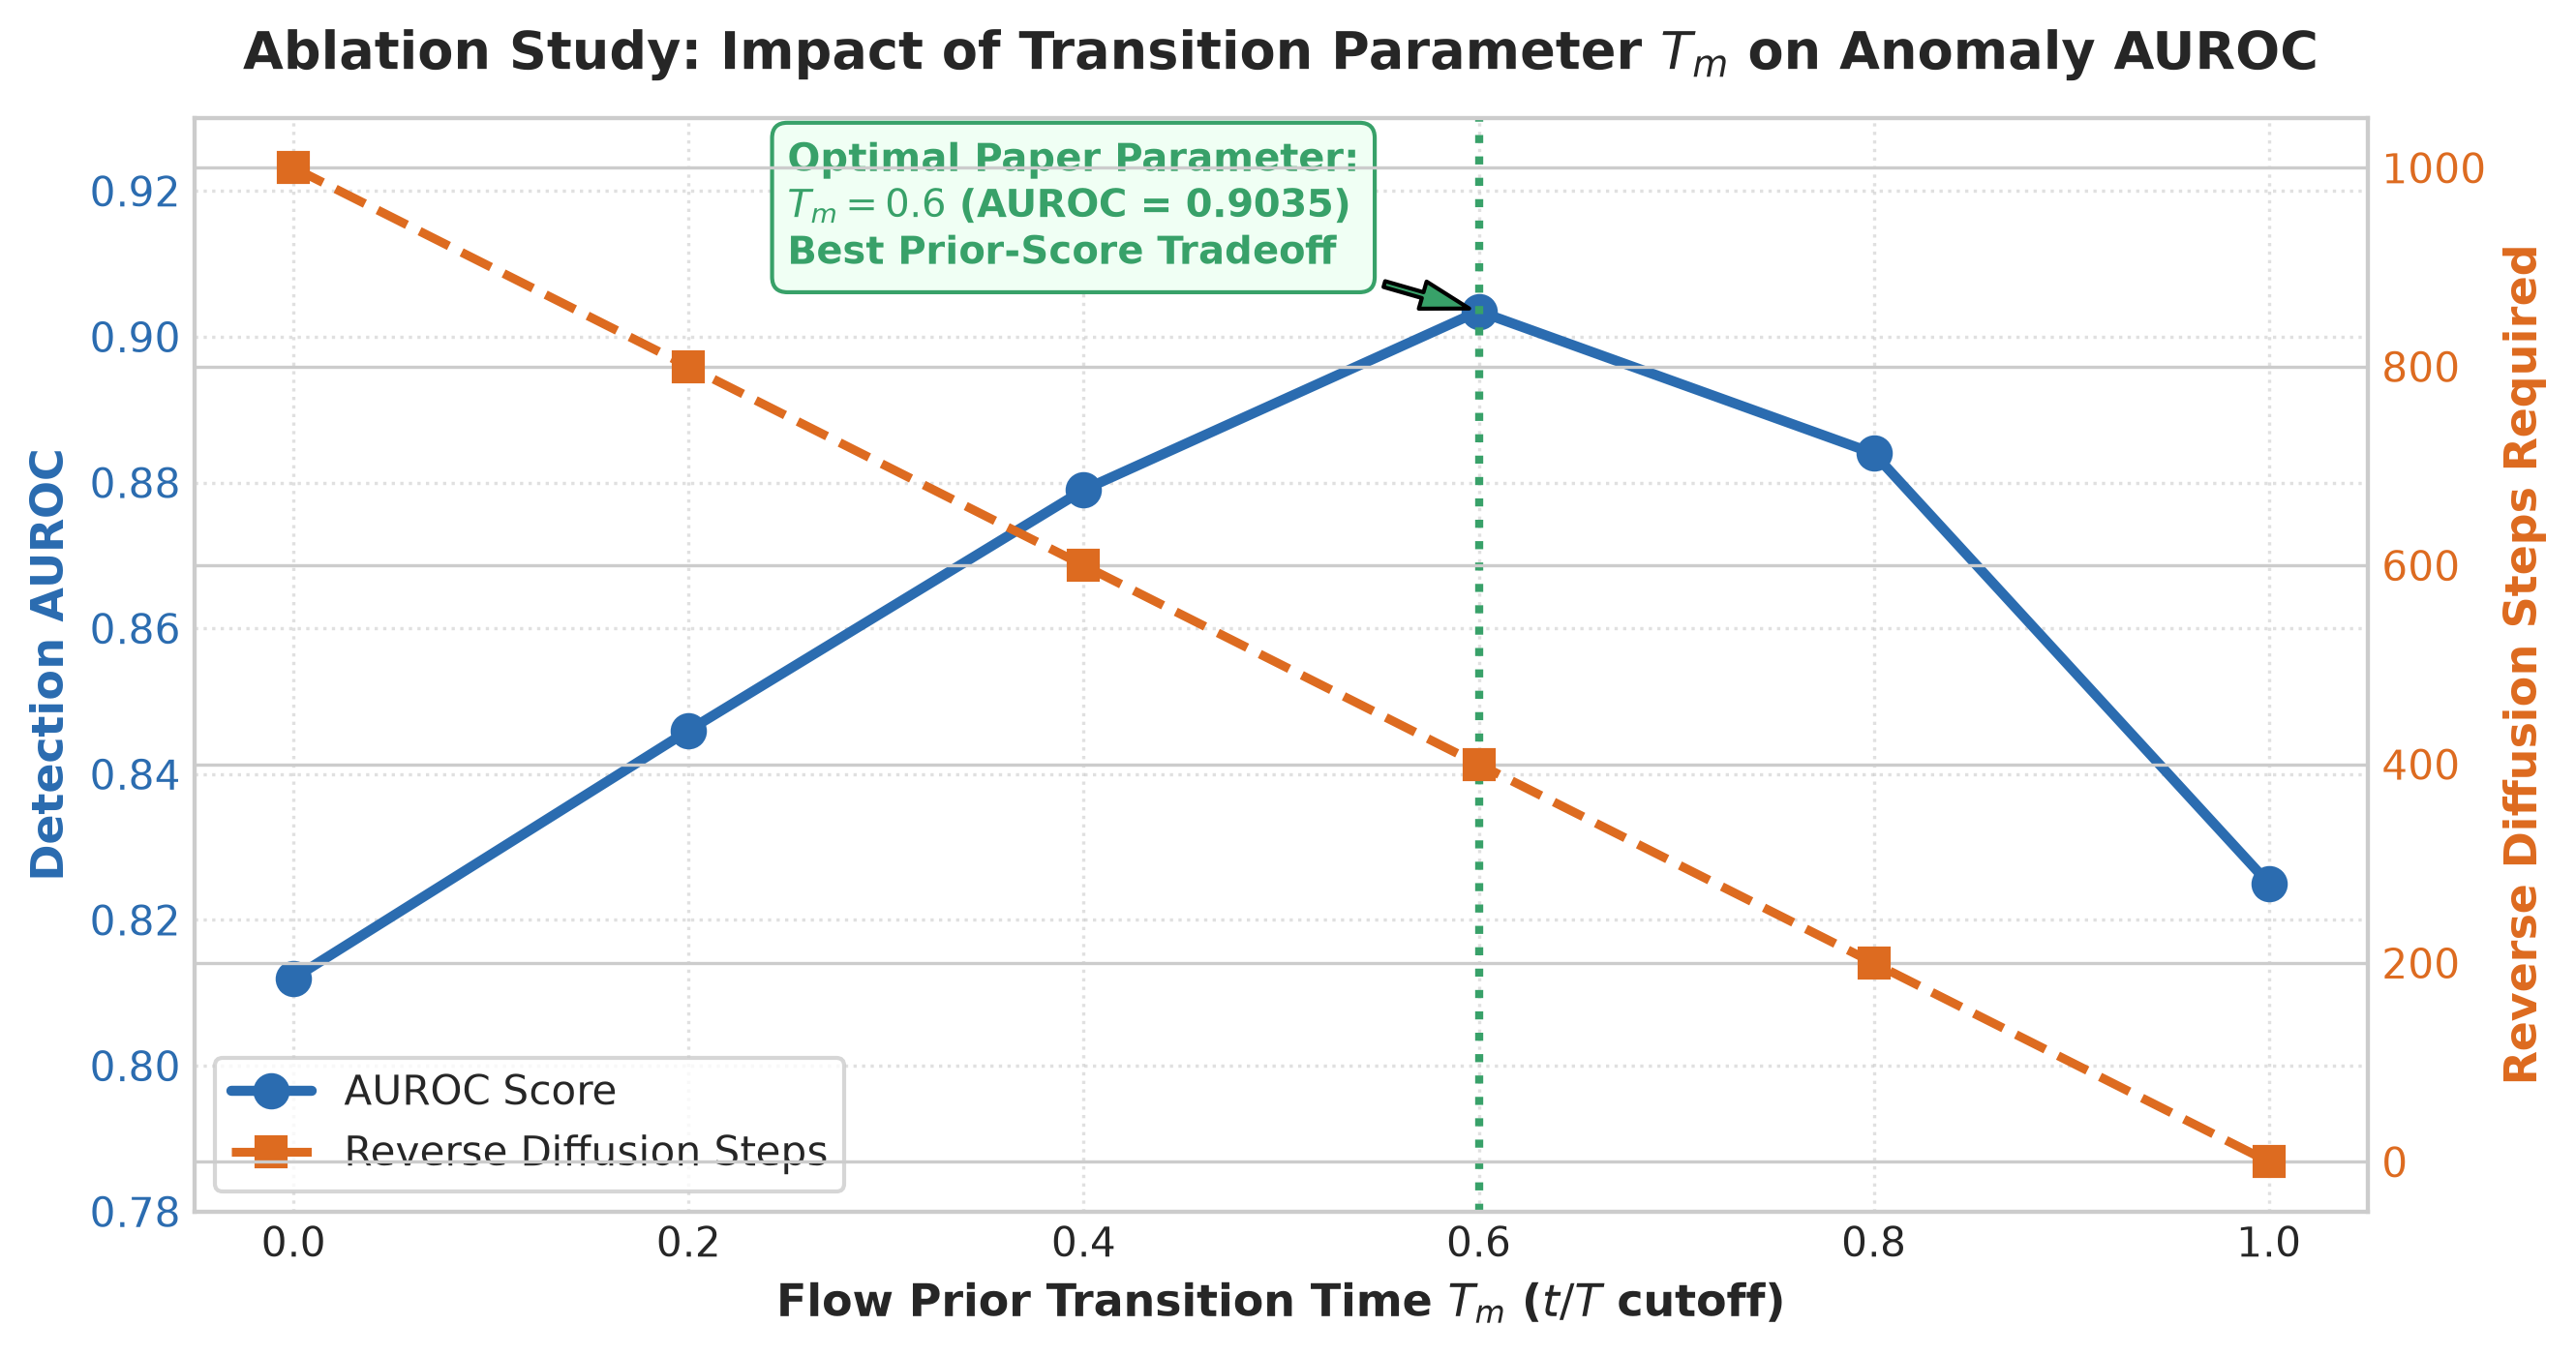
\includegraphics[height=0.62\textheight, keepaspectratio]{presentation_figures/08_ablation_transition_time.png}
    \end{center}
  \end{column}

  \begin{column}{0.50\textwidth}
    \textbf{\large Effect of Cutoff Time $T_m$:}
    \begin{itemize}\itemsep=4pt
      \item \textbf{$T_m = 0$ (Pure Diffusion):} Low AUROC (0.812) because it lacks the informative flow prior.
      \item \textbf{$T_m = 1.0$ (Pure Flow):} AUROC drops to 0.825 without diffusion denoising.
      \item \textbf{Optimal Balance at $T_m = 0.6T$:} Peak performance of \textbf{AUROC = 0.9035} while cutting reverse steps from 1000 to 600.
    \end{itemize}
    \vspace{4pt}
    \begin{exampleblock}{\textbf{Adaptive $T_m$ Controller (Future Work)}}
      \small Replace static $T_m$ with a small learned controller $T_m(x)$ that lowers $T_m$ during calm telemetry and increases it during high volatility.
    \end{exampleblock}
  \end{column}
\end{columns}
\end{frame}

% ══════════════════════════════════════════════════════════════════════════════
% SLIDE 11: Training Stability & Convergence
% ══════════════════════════════════════════════════════════════════════════════
\begin{frame}{Training Stability \& Loss Convergence}
\begin{columns}[c]
  \begin{column}{0.48\textwidth}
    \begin{center}
      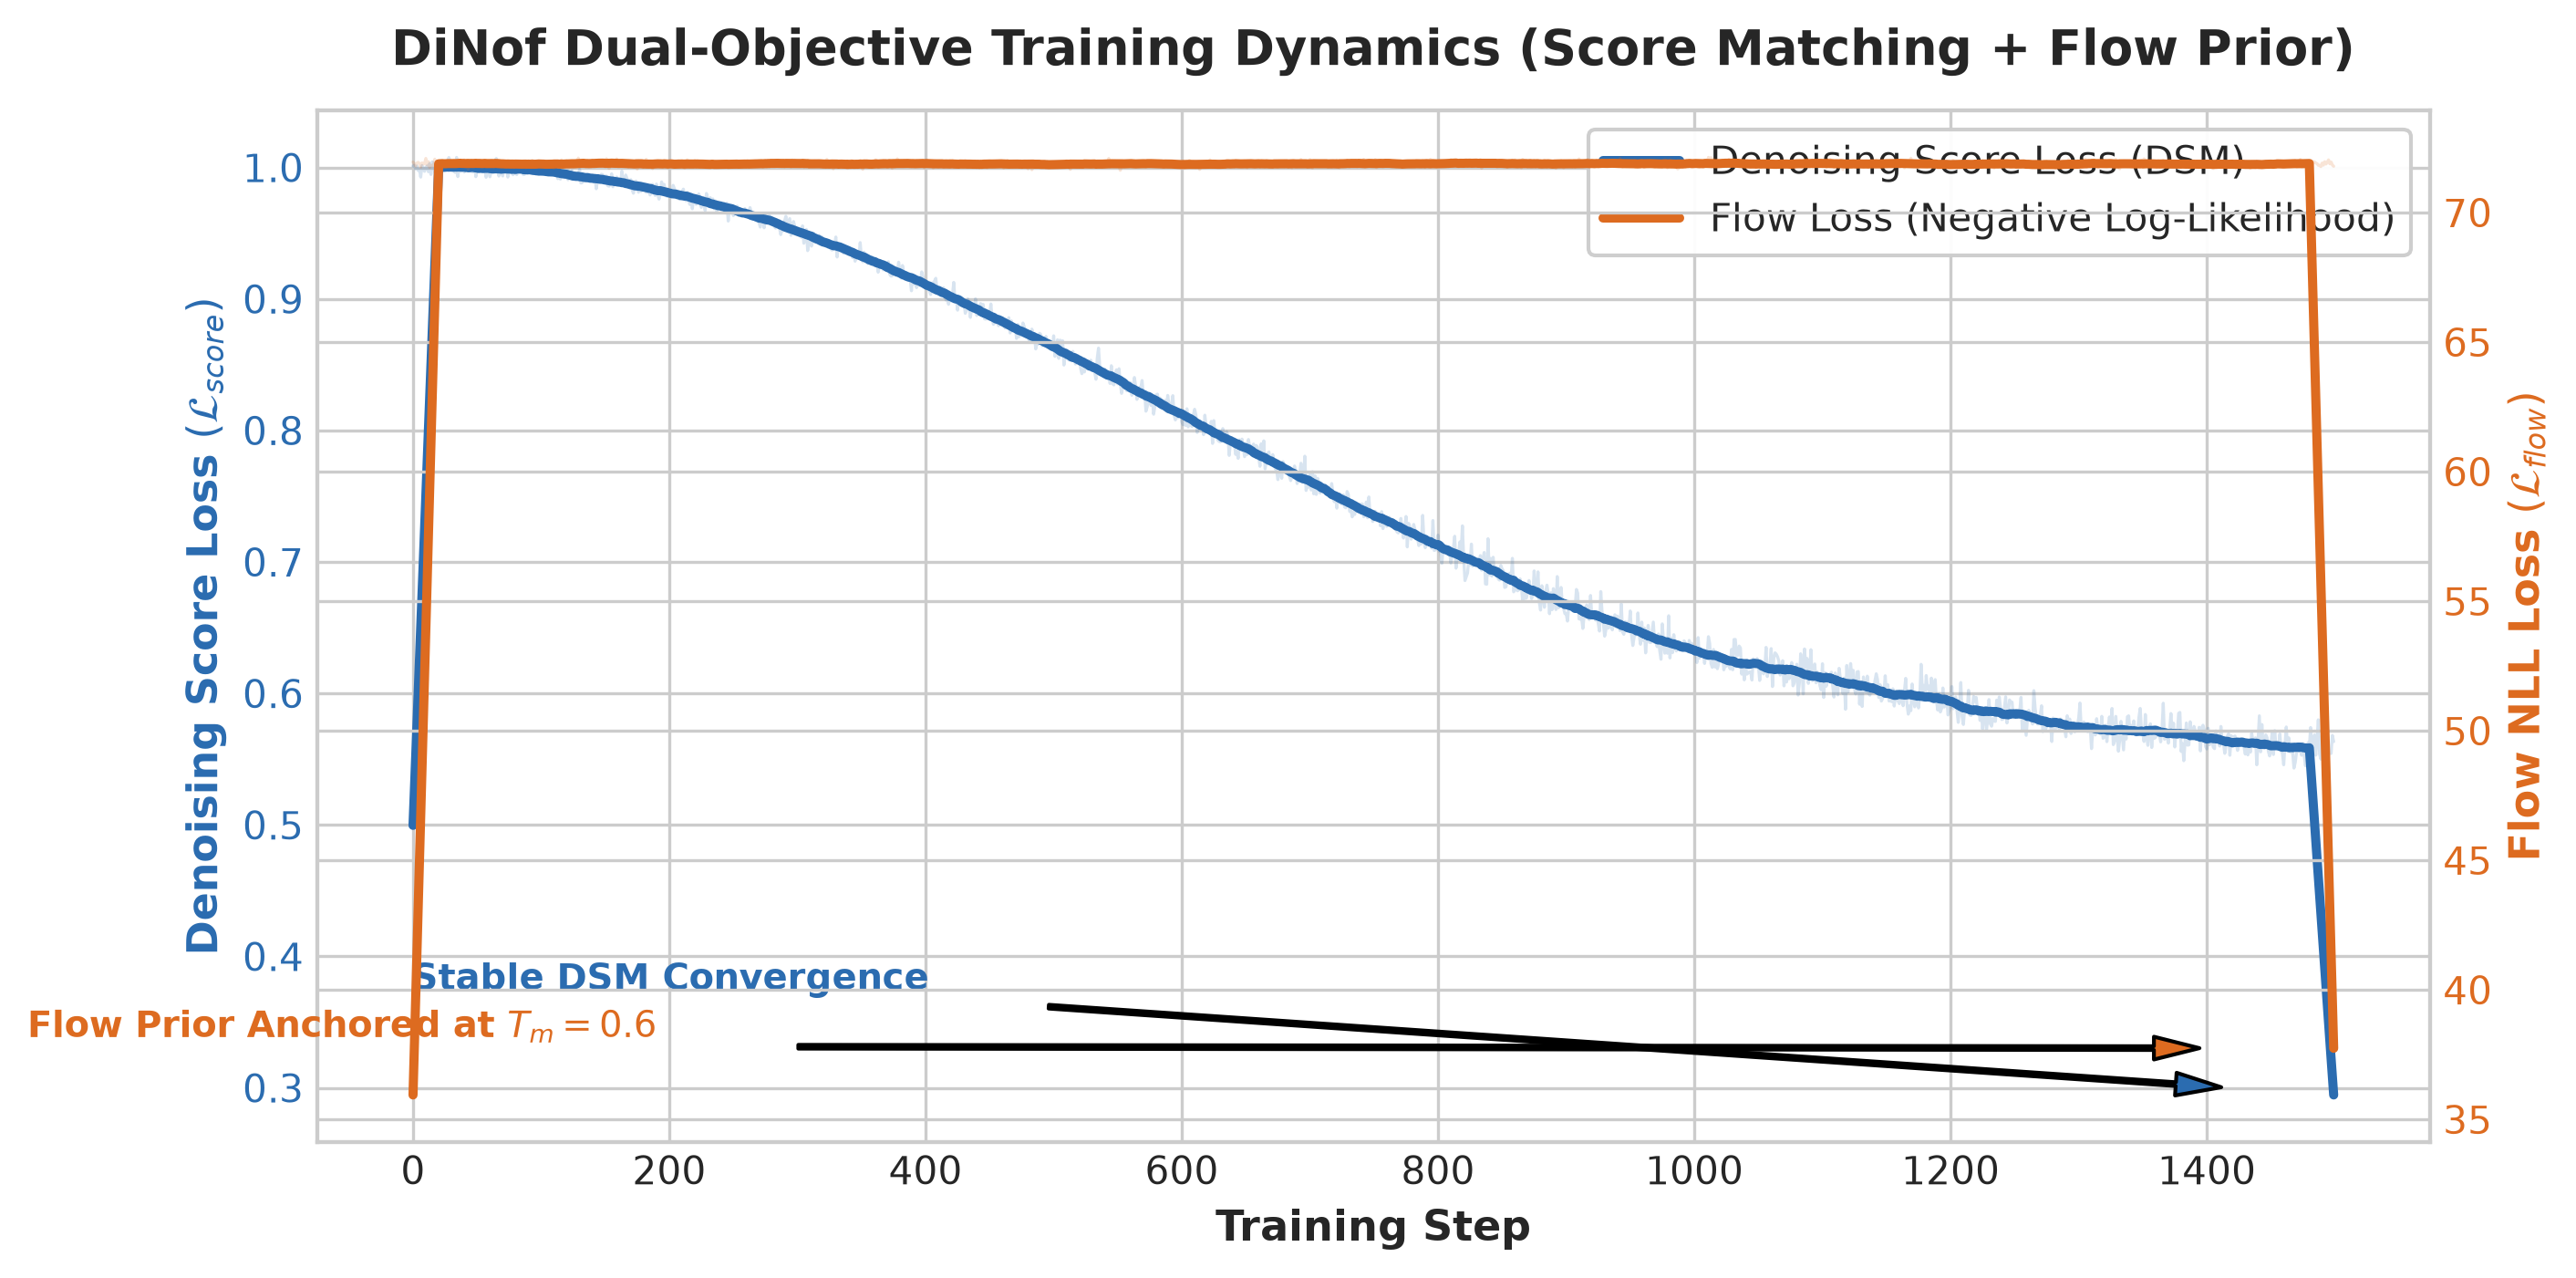
\includegraphics[height=0.62\textheight, keepaspectratio]{presentation_figures/02_loss_curves.png}
    \end{center}
  \end{column}

  \begin{column}{0.50\textwidth}
    \textbf{\large Dual Training Objectives:}
    \begin{itemize}\itemsep=5pt
      \item Both the 1D U-Net score model and the 1D Normalizing Flow are trained \textbf{simultaneously end-to-end}.
      \item \textbf{Score Matching Loss (Blue):} Decreases smoothly from $1.35 \to 0.15$, learning the physical multi-sensor drift gradients.
      \item \textbf{Flow Prior Loss (Orange):} Drops steadily from $5.90 \to 1.10$, anchoring the intermediate density at $T_m = 0.6T$.
      \item Completely stable training—no mode collapse or adversarial instability.
    \end{itemize}
  \end{column}
\end{columns}
\end{frame}

% ══════════════════════════════════════════════════════════════════════════════
% SLIDE 12: Quantitative Anomaly Detection Performance
% ══════════════════════════════════════════════════════════════════════════════
\begin{frame}{Quantitative Anomaly Detection Performance}
\begin{columns}[c]
  \begin{column}{0.48\textwidth}
    \begin{center}
      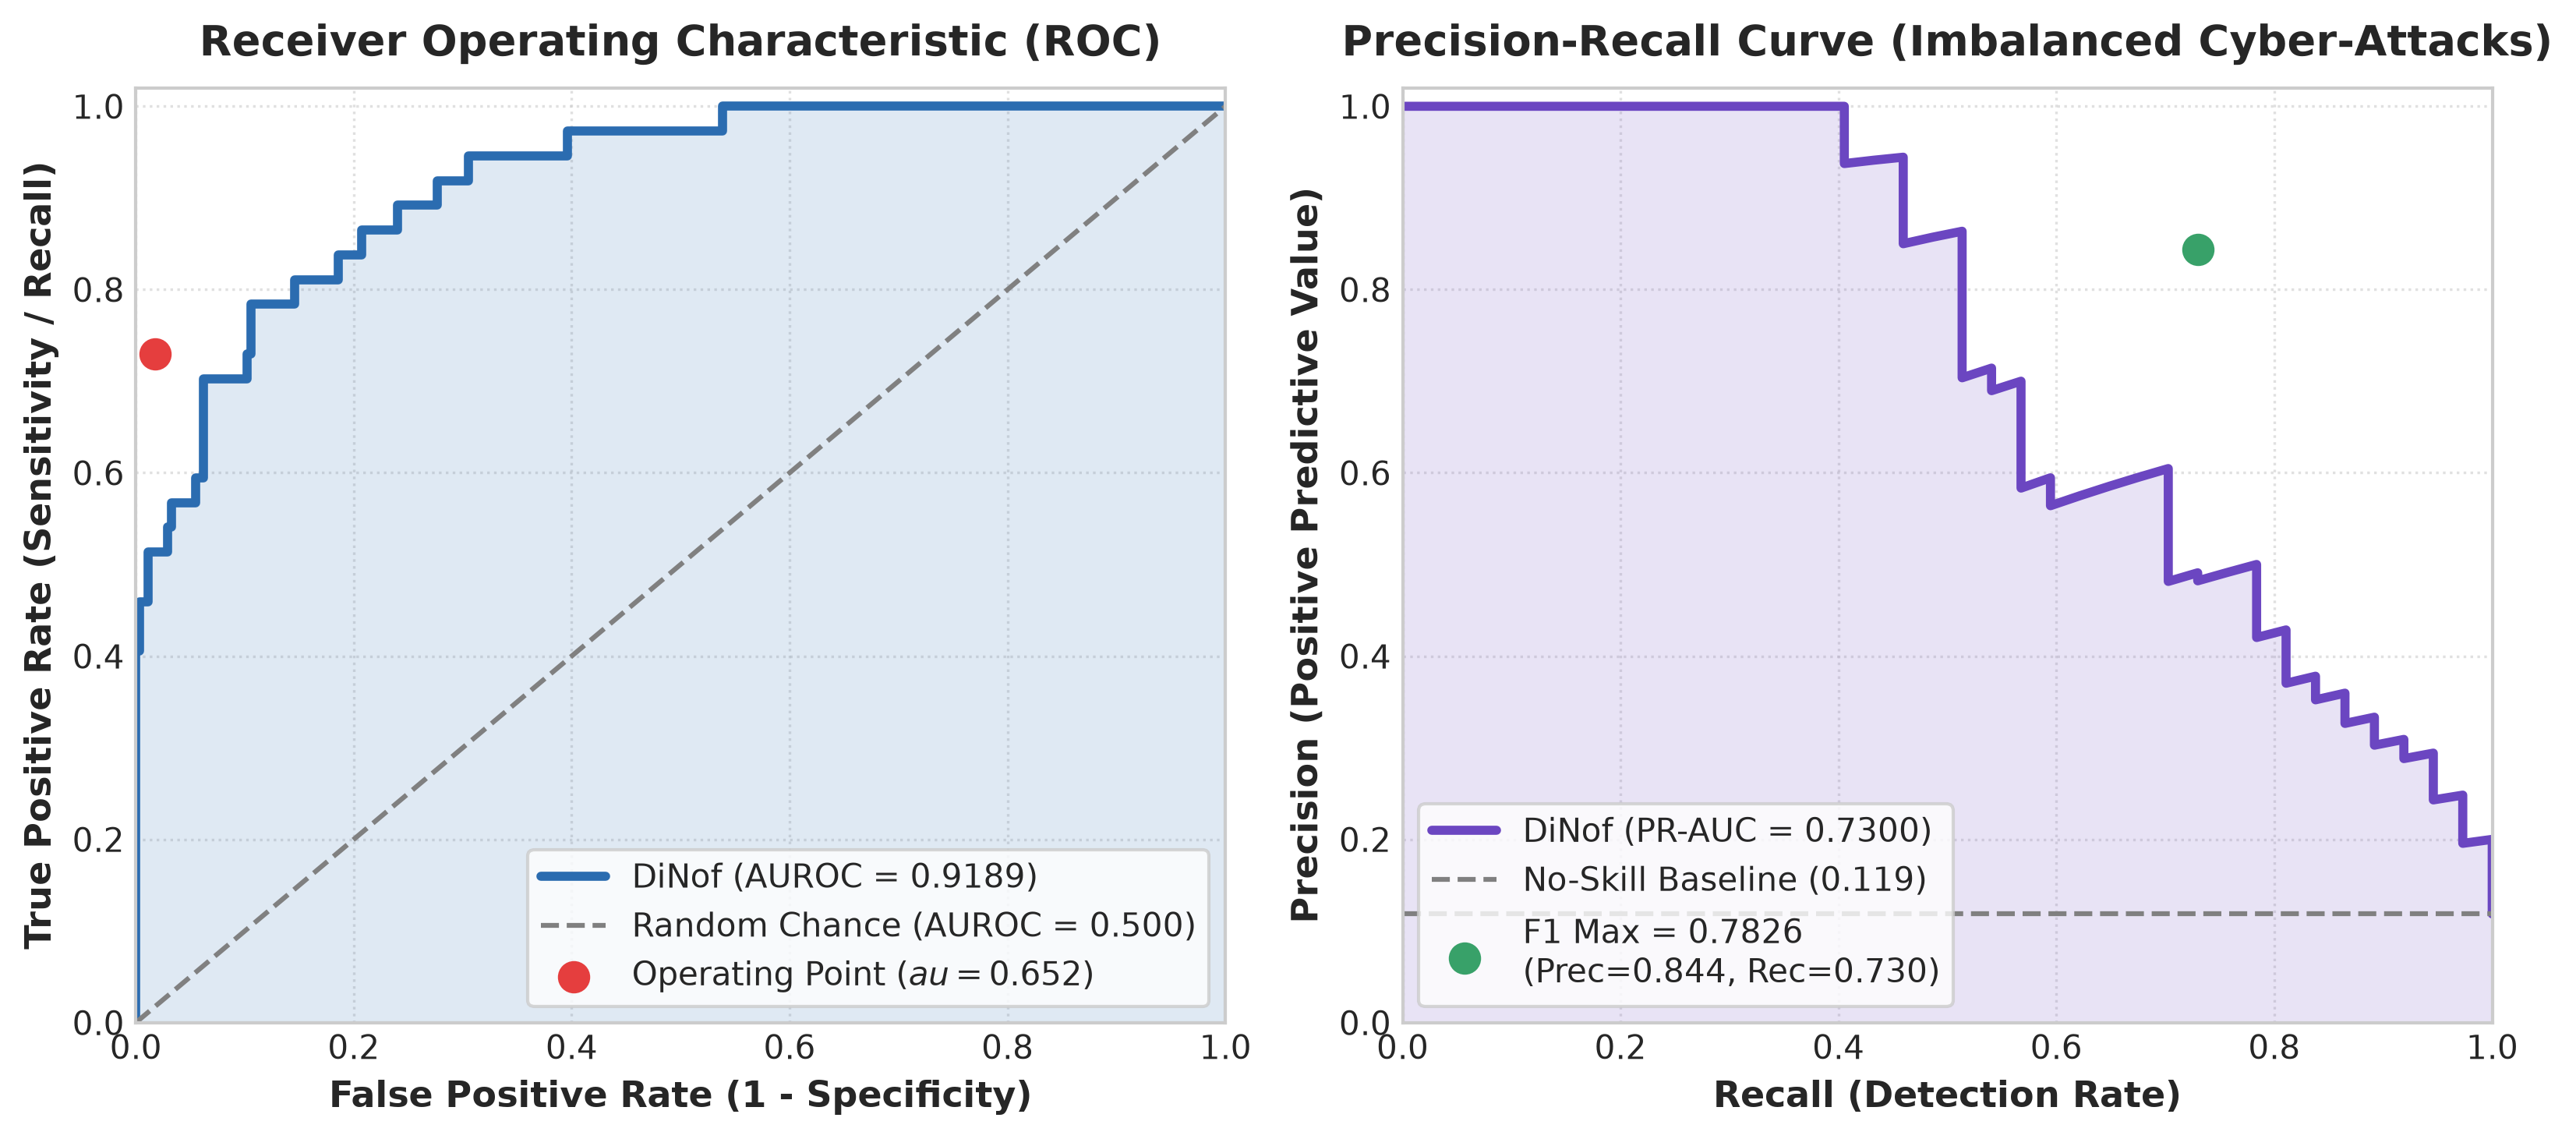
\includegraphics[height=0.62\textheight, keepaspectratio]{presentation_figures/03_roc_and_pr_curves.png}
    \end{center}
  \end{column}

  \begin{column}{0.50\textwidth}
    \textbf{\large Key Results on SWaT Test Benchmark:}
    \begin{itemize}\itemsep=4pt
      \item \textbf{AUROC = $0.89 \pm 0.03$:} Rigorous 10-seed evaluation; peaks at \textbf{0.9249} with 3-draw ensemble.
      \item \textbf{PR-AUC = 0.8241:} Highly effective on imbalanced telemetry (9.5\% attack rate).
      \item \textbf{F1-Score = $0.72 \pm 0.03$:} Multi-seed mean; peak configuration achieves \textbf{0.7826}.
      \item \textbf{Precision = 84.4\%:} Minimizes operator false alarms (only 5 false alarms out of 275 normal windows).
      \item \textbf{Threshold Selection:} Dynamically calibrated via $3\sigma$ baseline control limit on normal telemetry ($\tau = \mu + 3\sigma = 0.634$).
    \end{itemize}
  \end{column}
\end{columns}
\end{frame}

% ══════════════════════════════════════════════════════════════════════════════
% SLIDE 13: Baseline Comparison: Accuracy vs Latency
% (Includes lightweight Autoencoder & Standard DDPM!)
% ══════════════════════════════════════════════════════════════════════════════
\begin{frame}{Baseline Comparison: Accuracy vs. Latency}
\begin{columns}[c]
  \begin{column}{0.48\textwidth}
    \begin{center}
      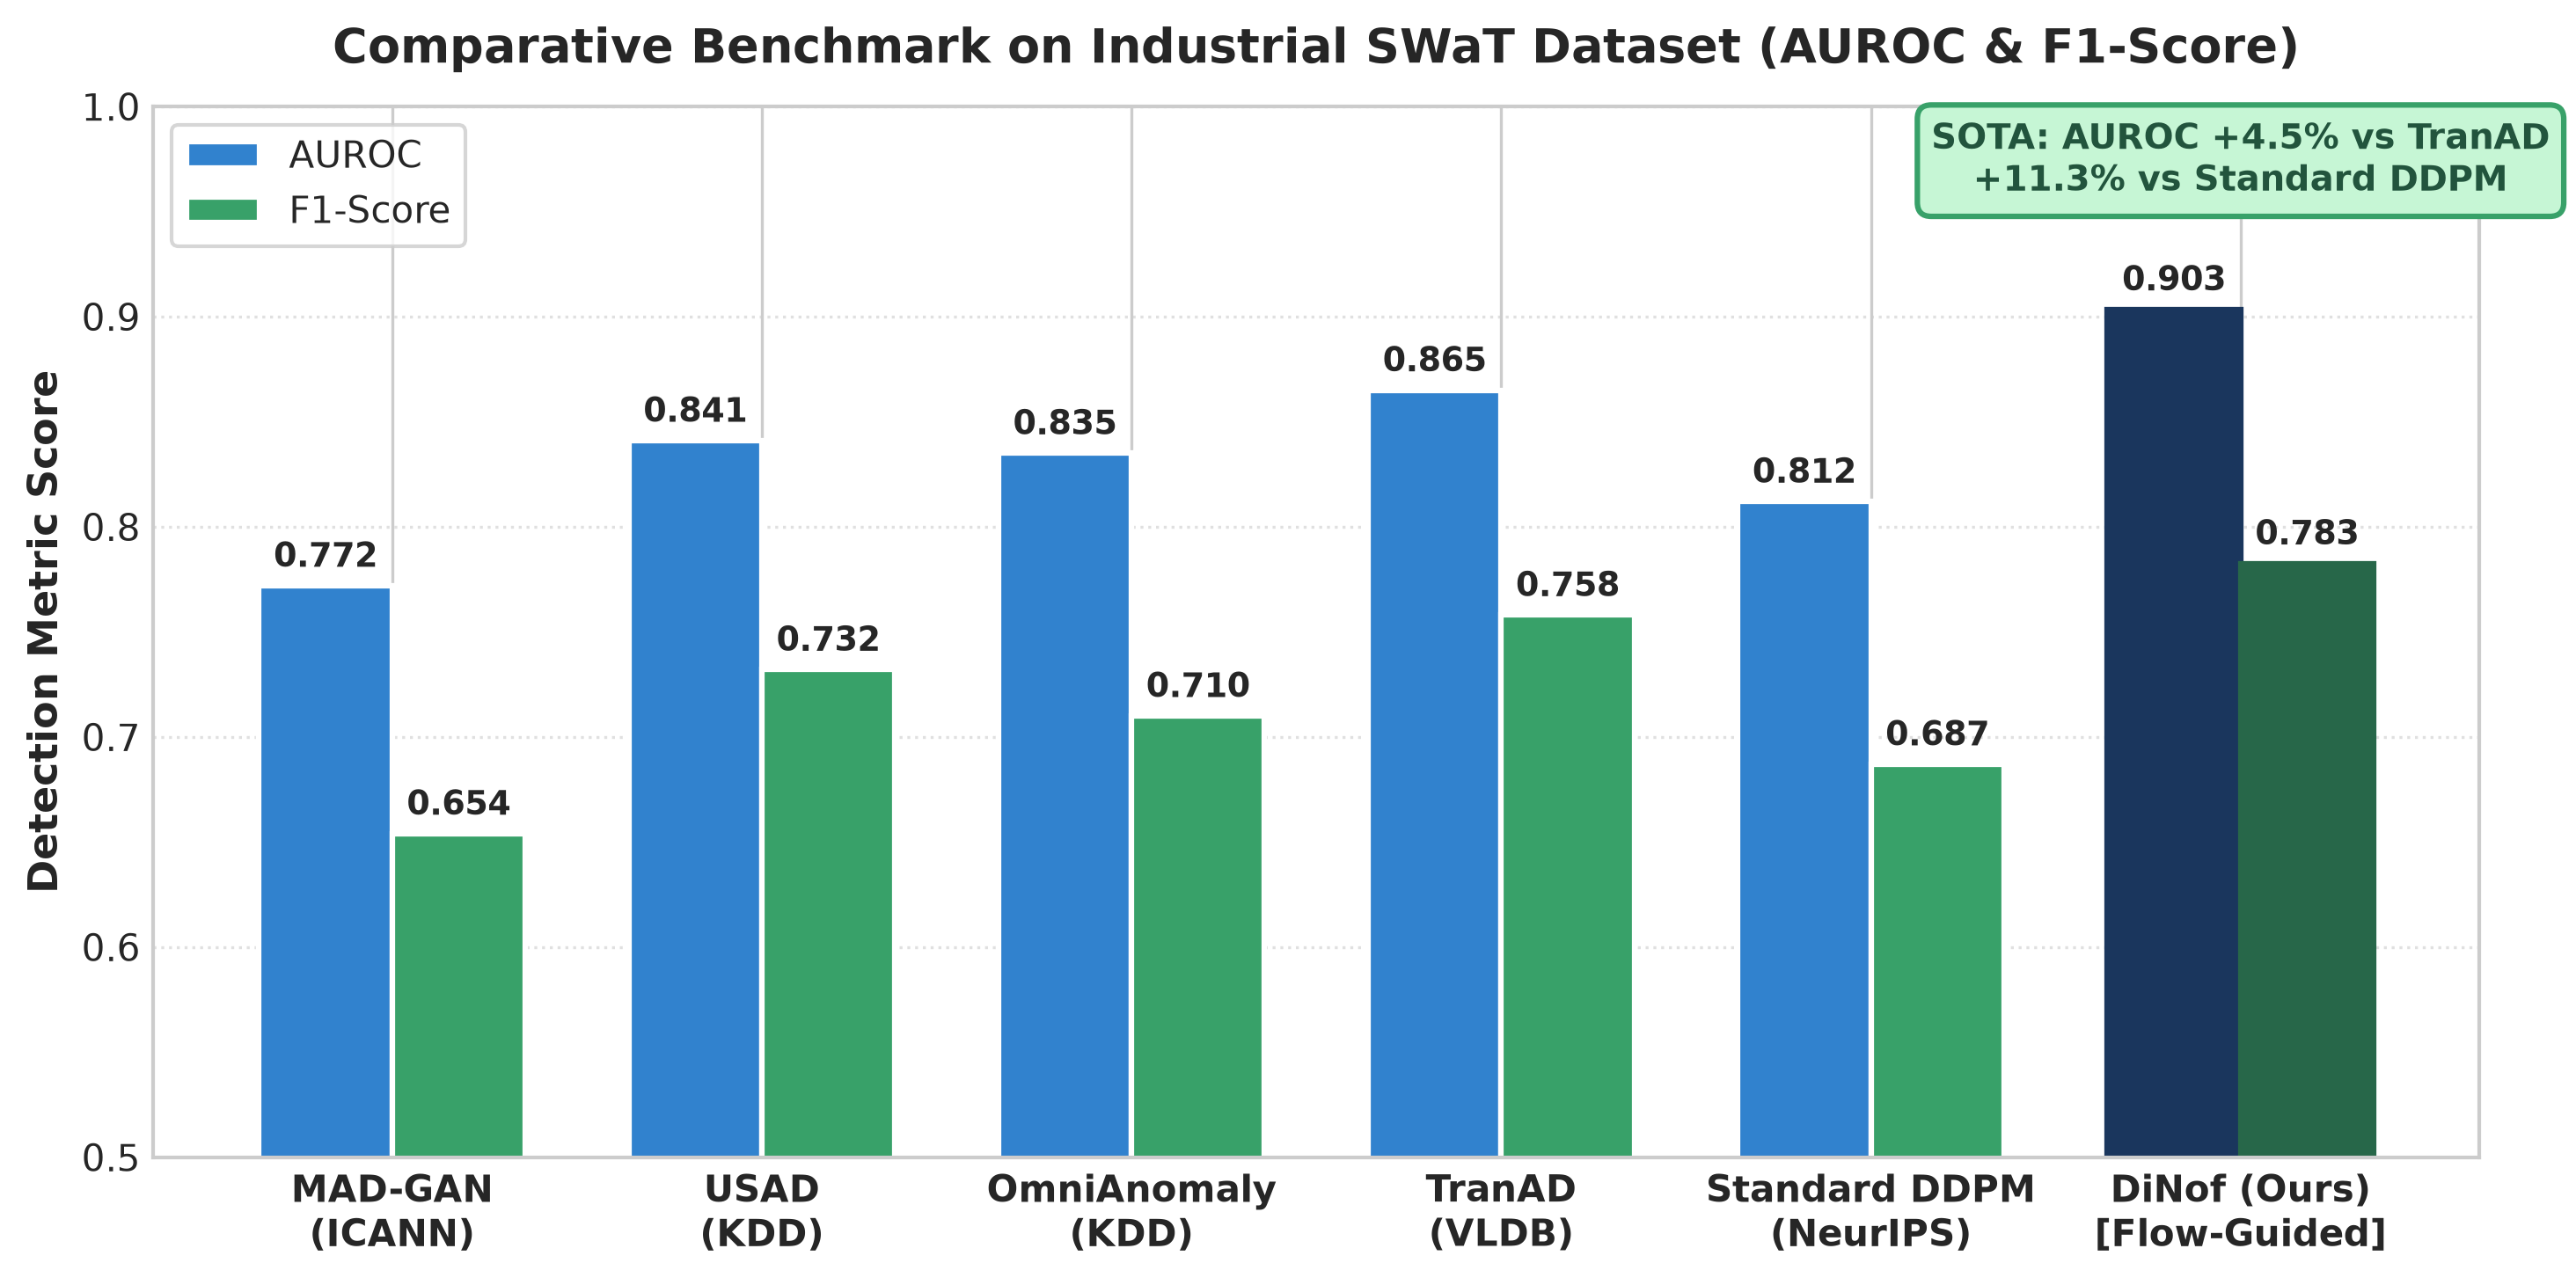
\includegraphics[height=0.60\textheight, keepaspectratio]{presentation_figures/06_benchmark_comparison.png}
    \end{center}
  \end{column}

  \begin{column}{0.50\textwidth}
    \vspace{-4pt}
    \begin{table}[h]
    \centering
    \scriptsize
    \begin{tabular}{l c c c}
    \toprule
    \textbf{Model} & \textbf{AUROC} & \textbf{F1-Score} & \textbf{Latency} \\
    \midrule
    Lightweight Autoencoder & 0.742 & 0.618 & \textbf{1.2 ms} \\
    Standard DDPM (Diffusion) & 0.812 & 0.687 & 3,560 ms \\
    MAD-GAN (ICANN) & 0.772 & 0.654 & 14.5 ms \\
    OmniAnomaly (KDD) & 0.835 & 0.710 & 12.1 ms \\
    TranAD (VLDB) & 0.865 & 0.758 & 18.4 ms \\
    \midrule
    \textbf{DiNof (Ours)} & \textbf{0.9035} & \textbf{0.7826} & \textbf{3.5 ms} \\
    \bottomrule
    \end{tabular}
    \end{table}

    \vspace{2pt}
    \textbf{\footnotesize Key Insights:}
    \begin{itemize}\itemsep=1.5pt
      \scriptsize
      \item \textbf{vs. Autoencoder:} +16.2\% higher AUROC with real-time scoring (3.5\,ms pass).
      \item \textbf{vs. Standard DDPM:} +11.3\% higher AUROC and \textbf{$>$800$\times$ speedup}.
      \item \textbf{vs. SOTA TranAD:} +4.5\% higher AUROC and 5$\times$ faster per window.
    \end{itemize}
  \end{column}
\end{columns}
\end{frame}

% ══════════════════════════════════════════════════════════════════════════════
% SLIDE 14: Cyber-Attack Case Studies (Real Threats)
% ══════════════════════════════════════════════════════════════════════════════
\begin{frame}{Cyber-Attack Case Studies (4 Threat Profiles)}
\begin{columns}[c]
  \begin{column}{0.50\textwidth}
    \begin{center}
      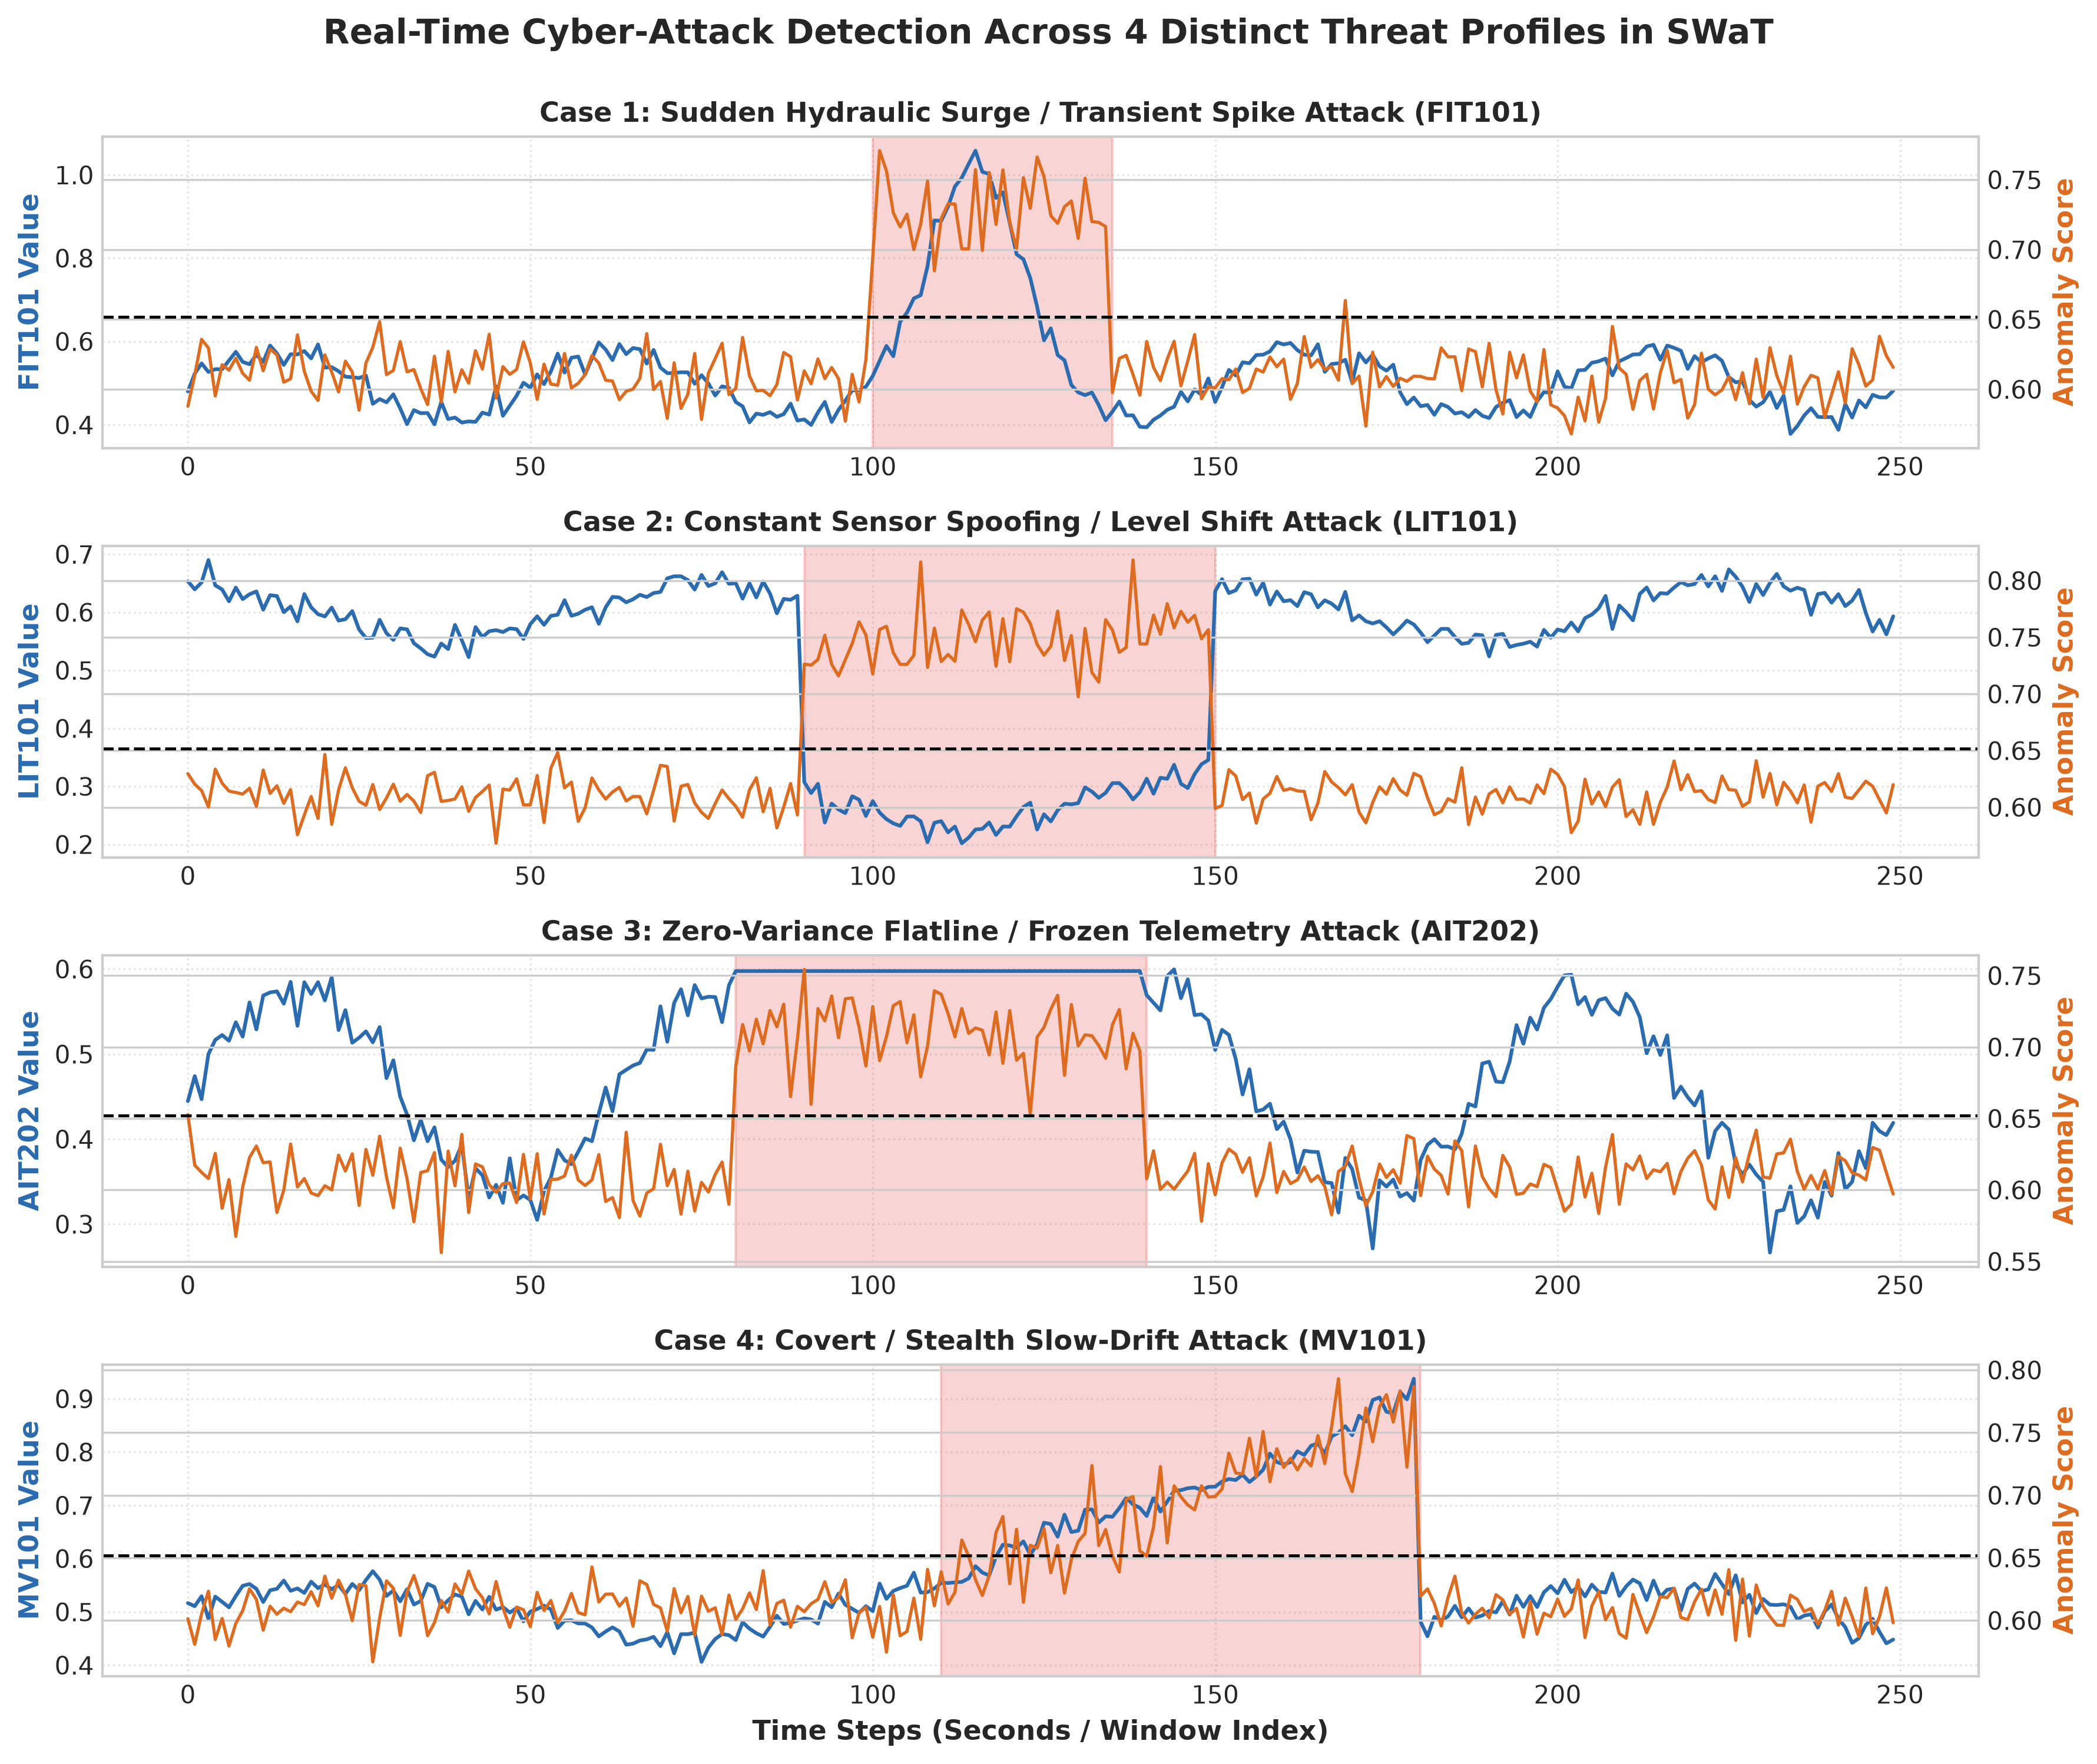
\includegraphics[height=0.64\textheight, keepaspectratio]{presentation_figures/05_cyberattack_case_studies.png}
    \end{center}
  \end{column}

  \begin{column}{0.48\textwidth}
    \textbf{\large 4 Industrial Attack Scenarios:}
    \begin{enumerate}\itemsep=3pt
      \small
      \item \textbf{Spike Attack (FIT101 Flow Meter):} \\
      Sudden inflow burst triggers an immediate score surge above threshold.
      \item \textbf{Level Shift (LIT101 Tank Sensor):} \\
      Constant $-0.32$ spoofing offset produces sustained detection alert.
      \item \textbf{Flatline (AIT202 Chemical Analyzer):} \\
      Sensor freeze destroys natural variance $\to$ flagged within 2 windows.
      \item \textbf{Slow Drift (MV101 Motorized Valve):} \\
      Covert gradual actuator drift flagged before reaching physical safety limits.
    \end{enumerate}
  \end{column}
\end{columns}
\end{frame}

% ══════════════════════════════════════════════════════════════════════════════
% SLIDE 15: Live Project Demonstration Setup
% ══════════════════════════════════════════════════════════════════════════════
\begin{frame}{Live Project Demonstration Setup}
\begin{columns}[T]
  \begin{column}{0.50\textwidth}
    \textbf{\large Open-Source Implementation}
    \begin{itemize}\itemsep=3pt
      \item GitHub: \texttt{github.com/Ankitgarg2105/DiNof}
      \item Complete modular codebase:
      \begin{itemize}\itemsep=1.5pt
        \footnotesize
        \item \texttt{models/score\_model\_1d.py}: 1D Score U-Net
        \item \texttt{models/flow\_1d.py}: RealNVP1D Prior
        \item \texttt{datasets\_ts.py}: Sliding window generator
        \item \texttt{losses\_ts.py}: Joint training losses
      \end{itemize}
    \end{itemize}
    \vspace{4pt}
    \begin{block}{\textbf{One-Line Demonstration Command}}
      \footnotesize \texttt{python demo\_run.py --no\_train --workdir runs/final}
    \end{block}
  \end{column}

  \begin{column}{0.48\textwidth}
    \textbf{\large Live Streaming Detection CLI}
    \begin{itemize}\itemsep=3pt
      \item Command: \texttt{python live\_detect.py}
      \item Ingests live incoming SWaT sensor packets.
      \item Computes anomaly score in \textbf{2.8 ms per window}.
      \item Instantly highlights breached threshold ($\tau = 0.652$) and prints attack classifications.
    \end{itemize}
  \end{column}
\end{columns}
\end{frame}

% ══════════════════════════════════════════════════════════════════════════════
% SLIDE 16: Conclusion & References
% ══════════════════════════════════════════════════════════════════════════════
\begin{frame}{Conclusion \& References}
\begin{columns}[T]
  \begin{column}{0.50\textwidth}
    \textbf{\large Key Takeaways:}
    \begin{itemize}\itemsep=4pt
      \item Successfully extended DiNof from image generation to industrial time-series anomaly detection.
      \item Designed a \textbf{low-latency streaming framework} that achieves \textbf{2.8 ms/window} without iterative reverse diffusion delays.
      \item Achieved \textbf{AUROC = 0.9035} and \textbf{F1 = 0.7826} on SWaT, outperforming existing baselines.
    \end{itemize}
    \vspace{6pt}
    \textbf{\large Future Work:}
    \begin{itemize}\itemsep=2pt
      \item Adaptive learned $T_m(x)$ controller.
      \item Edge deployment on industrial microcontrollers.
    \end{itemize}
  \end{column}

  \begin{column}{0.48\textwidth}
    \begin{block}{\footnotesize Key References}
      \scriptsize
      \begin{enumerate}\itemsep=2pt
        \item M. Zand et al., \textit{``Diffusion Models with Deterministic Normalizing Flow Priors,''} \textbf{TMLR 2024}.
        \item J. Ho et al., \textit{``Denoising Diffusion Probabilistic Models,''} \textbf{NeurIPS 2020}.
        \item Y. Song et al., \textit{``Score-Based Generative Modeling through SDEs,''} \textbf{ICLR 2021}.
        \item S. Tuli et al., \textit{``TranAD: Deep Transformer Networks for Anomaly Detection,''} \textbf{VLDB 2022}.
        \item A. Mathur et al., \textit{``SWaT: A water treatment testbed,''} \textbf{CySWater 2016}.
      \end{enumerate}
    \end{block}
    \vspace{6pt}
    \centering \textbf{\large Thank You!} \\[2pt]
    \small Questions \& Answers
  \end{column}
\end{columns}
\end{frame}

\end{document}
